\chapter{差速扫地机器人：先约束运动方向}
\begin{notebox}
\textbf{目标}\quad 从左右轮速得到圆心位姿，理解不能横移的含义。\\
\textbf{范围}\quad 独立无滑移运动学实验；主线仍为全向圆盘，未接入轮力矩或 NMPC。
\end{notebox}
\section{圆盘外形相同，能做的动作不同}
若希望先学建图与轨迹优化，全向圆盘能把问题分开；若研究扫地机器人，差速模型更贴近驱动约束。
圆盘半径仍负责碰撞，车轮半径 $r_w$ 和左右接地点间距 $b$ 则负责运动换算，三者不要混用。
轮速 $w_L,w_R$ 单位为 rad/s，同号为前进，理想无滑移模型为
\begin{equation}
 v=\frac{r_w(w_R+w_L)}2,\quad
 \omega=\frac{r_w(w_R-w_L)}b,\qquad
 \dot x=v\cos\psi,\quad\dot y=v\sin\psi,\quad\dot\psi=\omega.
\end{equation}
横向速度满足 $-\sin\psi\,\dot x+\cos\psi\,\dot y=0$。
它约束瞬时速度，不能写成一个简单的位置等式消掉；因此称为非完整约束。
机器人可以通过前进和转向改变横向位置，但不能直接侧移。

\lstinputlisting[language=C++,linerange={differential_kinematics_begin-differential_kinematics_end},
 includerangemarker=false]{../ros2_ws/src/motion2d/src/sim/differential_drive.cpp}
stepDifferential 复用第 04 章恒定机体系速度的精确 SE(2) 积分，避免另写一套近似积分器。
本函数没有电机、轮胎滑移或质量；阶跃轮速也不能凭空生成物理正确的瞬时 IMU 加速度。

\section{手算一次圆弧}
取 $r_w=0.05$ m、$b=0.4$ m、$w_L=2$、$w_R=6$ rad/s，
得到 $v=0.2$ m/s、$\omega=0.5$ rad/s、转弯半径 $v/\omega=0.4$ m。
从原点、yaw=0 出发，$t=\pi$ s 时应到达 $(0.4,0.4)$ m、yaw=$\pi/2$；
$t=4\pi$ s 恰好一圈。速度初始样本为施加轮速前的静止状态，随后为保持命令的运动学状态。

\clearpage
\begin{lstlisting}[language=bash]
ros2 run motion2d differential_drive_demo > textbook/data/appB_circle.csv
/usr/bin/python3 scripts/plot_appB.py
\end{lstlisting}
\begin{figure}[!ht]
\centering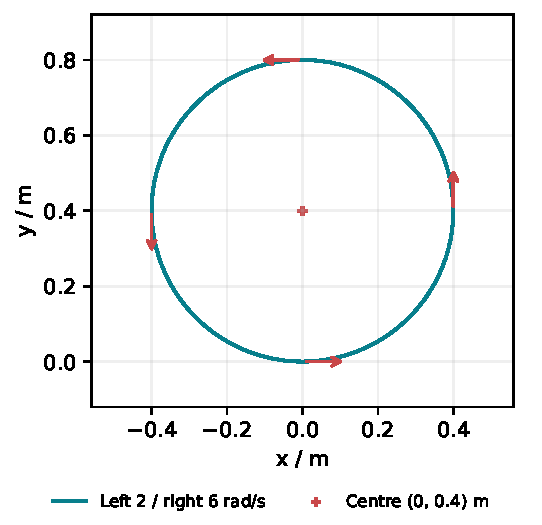
\includegraphics[width=.69\linewidth]{figures/appB_circle.pdf}
\caption{实际积分得到的圆弧，坐标等比例；箭头表示朝向，始终与运动方向相切。
这是独立几何实验，不包含障碍、轮动力学或 ROS 轨迹跟踪。}
\end{figure}

\section{怎样接到轨迹与控制}
对非零、正向运动的平滑参考 $p(t)$，可从速度与加速度计算
\begin{equation}
 \psi=\operatorname{atan2}(v_y,v_x),\qquad v=\|\dot p\|,\qquad
 \omega=\frac{v_xa_y-v_ya_x}{v_x^2+v_y^2},\qquad \kappa=\omega/v.
\end{equation}
此时 yaw 不能再独立任意指定。低速处上述分母接近零，停点和倒车必须定义单独的运动模式；
不能靠一个很小的分母下限，把不一致轨迹变成“可行”。原地旋转则应使用 $v=0$、左右反向轮速。

第 18 章预测矩阵是全向受力模型，直接换话题名不会变成差速控制。
一种扩展是以 $(x,y,\psi)$ 为状态、$(v,\omega)$ 为输入做 NMPC：在每次滚动优化中保留
三角函数运动方程，加入轮速及变化率限制，并在求解失败时制动。
若输入轮力矩，还应增加轮惯量、质量和轮地接触模型；这些扩展本课程未实现。

\paragraph{练习与验收}
appB-1 补全逆运动学，手算直行、倒车、原地转动与圆弧四组轮速。
核心测试另外检查四分之一圆解析解、分步积分一致性和零侧向速度。
改变两轮速的公共倍率，解释为何圆半径不变、转完一圈所需时间改变。
